\documentclass[a4paper]{report}
\usepackage[utf8]{inputenc}
\usepackage[T1]{fontenc}
\usepackage{RJournal}
\usepackage{amsmath,amssymb,array}
\usepackage{booktabs}


% tightlist command for lists without linebreak
\providecommand{\tightlist}{%
  \setlength{\itemsep}{0pt}\setlength{\parskip}{0pt}}


% Always define CSL refs as bib entries are contained in separate doc
% Pandoc citation processing
\newlength{\cslhangindent}
\setlength{\cslhangindent}{1.5em}
\newlength{\csllabelwidth}
\setlength{\csllabelwidth}{3em}
\newlength{\cslentryspacingunit} % times entry-spacing
\setlength{\cslentryspacingunit}{\parskip}
% for Pandoc 2.8 to 2.10.1
\newenvironment{cslreferences}%
  {}%
  {\par}
% For Pandoc 2.11+
\newenvironment{CSLReferences}[2] % #1 hanging-ident, #2 entry spacing
 {% don't indent paragraphs
  \setlength{\parindent}{0pt}
  % turn on hanging indent if param 1 is 1
  \ifodd #1
  \let\oldpar\par
  \def\par{\hangindent=\cslhangindent\oldpar}
  \fi
  % set entry spacing
  \setlength{\parskip}{#2\cslentryspacingunit}
 }%
 {}
\usepackage{calc}
\newcommand{\CSLBlock}[1]{#1\hfill\break}
\newcommand{\CSLLeftMargin}[1]{\parbox[t]{\csllabelwidth}{#1}}
\newcommand{\CSLRightInline}[1]{\parbox[t]{\linewidth - \csllabelwidth}{#1}\break}
\newcommand{\CSLIndent}[1]{\hspace{\cslhangindent}#1}



\begin{document}


%% do not edit, for illustration only
\sectionhead{Contributed research article}
\volume{14}
\volnumber{4}
\year{2022}
\month{December}
\setcounter{page}{223}

\begin{article}
  % !TeX root = RJwrapper.tex
\title{populR: a Package for Population Downscaling in R}
\author{by Marios Batsaris and Dimitris Kavroudakis}

\maketitle

\abstract{%
Population data provision is usually framed by regulations and restrictions and hence spatially aggregated in predefined enumeration units such as city blocks and census tracts. Many applications require population data at finer scale, and therefore, one may use downscaling methods to transform population counts from coarse spatial units into smaller ones. Although numerous methods for downscaling of population data have been reported in the scientific literature, only a limited number of implementation tools exist. In this study, we introduce populR, an R package that responds to this need. populR provides two downscaling methods, namely Areal Weighted Interpolation and Volume Weighted Interpolation, which are illustrated and compared to alternative implementations in the sf and areal packages using a case study from Mytilini, Greece. The results provide evidence that the vwi approach outperforms the others, and thus, we believe R users may gain significant advantage by using populR for population downscaling.
}

\hypertarget{introduction}{%
\section{Introduction}\label{introduction}}

Information about the spatial distribution of the population is crucial in addressing a wide range of geographical information science problems (Dobson et al. 2000; Ahola et al. 2007; Freire and Aubrecht 2012; Bian and Wilmot 2015; Calka, Nowak Da Costa, and Bielecka 2017; Batsaris et al. 2019; Bahadori, Gonçalves, and Moura 2021; Wang et al. 2021; Han, Hu, and Wang 2020). One of the most common sources of population data is the Census of Population (Tenerelli, Gallego, and Ehrlich 2015; Liu, Kyriakidis, and Goodchild 2008). In the EU, censuses are carried out every ten years and are regulated by the EU 763/2008 law (European Union 2009). During the census, detailed information about the population is collected with a high level of granularity. This information is confidential, and due to personal data laws and privacy concerns, census data are de-identified via spatial aggregation into coarse administrative units.

Aggregated representations of census data may not reflect the spatial heterogeneity of the population within the reported administrative units, and therefore, one may need to use downscaling methods to transform population counts from the predefined coarse boundaries (source) into finer-scale sub-units (target). Areal interpolation is broadly used in population downscaling (Tenerelli, Gallego, and Ehrlich 2015).

Areal interpolation methods can be categorized according to usage of additional information such as land use data and night lights to guide the interpolation process. Ancillary information independent methods are further distinguished in: a) point-based and b) area-based (Wu, Qiu, and Wang 2005; Comber and Zeng 2019). Areal Weighted Interpolation (\emph{AWI}) is one of the most common methods of areal interpolation of population without exploiting ancillary information {[}Comber and Zeng (2019); Kim and Yao (2010);{]} in a Geographic Information System (GIS). \emph{AWI} guides the interpolation process on the basis of areal weights calculated by the area of intersection between the source and target features (Goodchild and Lam 1980). This method has four main advantages: a) It is easy and straightforward to implement; b) it does not require ancillary information; c) it preserves the initial volume (i.e., the total population within the source zone); and d) it may be implemented in both vector and raster environments (Comber and Zeng 2019; Fisher and Langford 1995; Kim and Yao 2010; Lam 1983; Qiu, Zhang, and Zhou 2012). On the other hand, one of the main disadvantages of \emph{AWI} is its assumption of homogeneity within source zone features (Comber and Zeng 2019; Qiu, Zhang, and Zhou 2012).

\CRANpkg{sf} (Pebesma 2018) and \CRANpkg{areal} (Prener and Revord 2019) provide \emph{AWI} functionality in R. \CRANpkg{sf} comes up with a formula either for extensive (population) or intensive (population density) interpolation that calculates the areal weights based on the total area of the source features (\emph{total weights}), which makes it suitable for completely overlapping data. \CRANpkg{areal} extends sf functionality by providing an additional formula for weight calculation for data without complete overlap. In this case, areal weights are calculated using the sum of the remaining source areas after the intersection (\emph{sum weights}) (Prener and Revord 2019).

When the case involves downscaling of urban population data (small scale applications) where the source features (such as city blocks or census tracts) are somehow larger than target features (such as buildings) in terms of footprint area, the \CRANpkg{sf} functionality is unable to calculate the areal weights correctly. Additionally, \CRANpkg{areal} may be confusing for novice R (or GIS) users as it is not obvious that the weight option should be set to \emph{sum} to calculate areal weights properly.

To overcome such limitations, we introduce \CRANpkg{populR} (Batsaris 2022), a package for downscaling of population data using areal interpolation methods. \CRANpkg{populR} provides an \emph{AWI} approach that matches \CRANpkg{areal} functionality using \emph{sum weights} and a \emph{VWI} (Volume Weighted Interpolation) approach that uses the area of intersection between source and target features multiplied by the building height or number of floors (volume) to guide the interpolation process.

The remainder of the paper is structured as follows. The next section lists the methods included in the \CRANpkg{populR} package, further explains and demonstrates using examples. The numerical experiments section illustrates and discusses the results obtained by \CRANpkg{populR} and compares the results to other alternatives in R. Finally, the paper concludes with a summary, along with future improvements, in the conclusions section.

\hypertarget{the-populr-package}{%
\section{The populR package}\label{the-populr-package}}

\CRANpkg{populR} is available to R users through the CRAN and Github repositories and may be installed as shown in the code block below.

\begin{verbatim}
# CRAN installation
install.packages("populR")

# Github installation
devtools::install_github("mbatsaris/populR")
\end{verbatim}

The \CRANpkg{populR} functionality focuses on three main pillars, namely downscaling, rounding, and comparing. Additionally, sample data (objects of class \emph{sf} (Pebesma 2018)) representing city blocks, including population counts (\emph{src}) and individual buildings attributed by the number of floors (\emph{trg}) from a small part of the city of Mytilini, Greece, are also available for further experimentation with the package's functionality.

\hypertarget{downscaling}{%
\subsection{Downscaling}\label{downscaling}}

Population downscaling is carried out by the primary \texttt{pp\_estimate} function.

Suppose a set of \(j = 1, ..., J\) city block polygons (source) accompanied by population counts and an incongruent yet superimposed set of \(i = 1, ..., B_j\) individual building polygons (target), along with their characteristics such as footprint area and/or number of floors (or height), the \texttt{pp\_estimate}, aims to transform population counts from the source to the target using \emph{AWI} and \emph{VWI} approaches. The mathematics behind both approaches is presented in the next two subsections and graphically illustrated in figure \ref{fig:methods}.

\begin{figure}
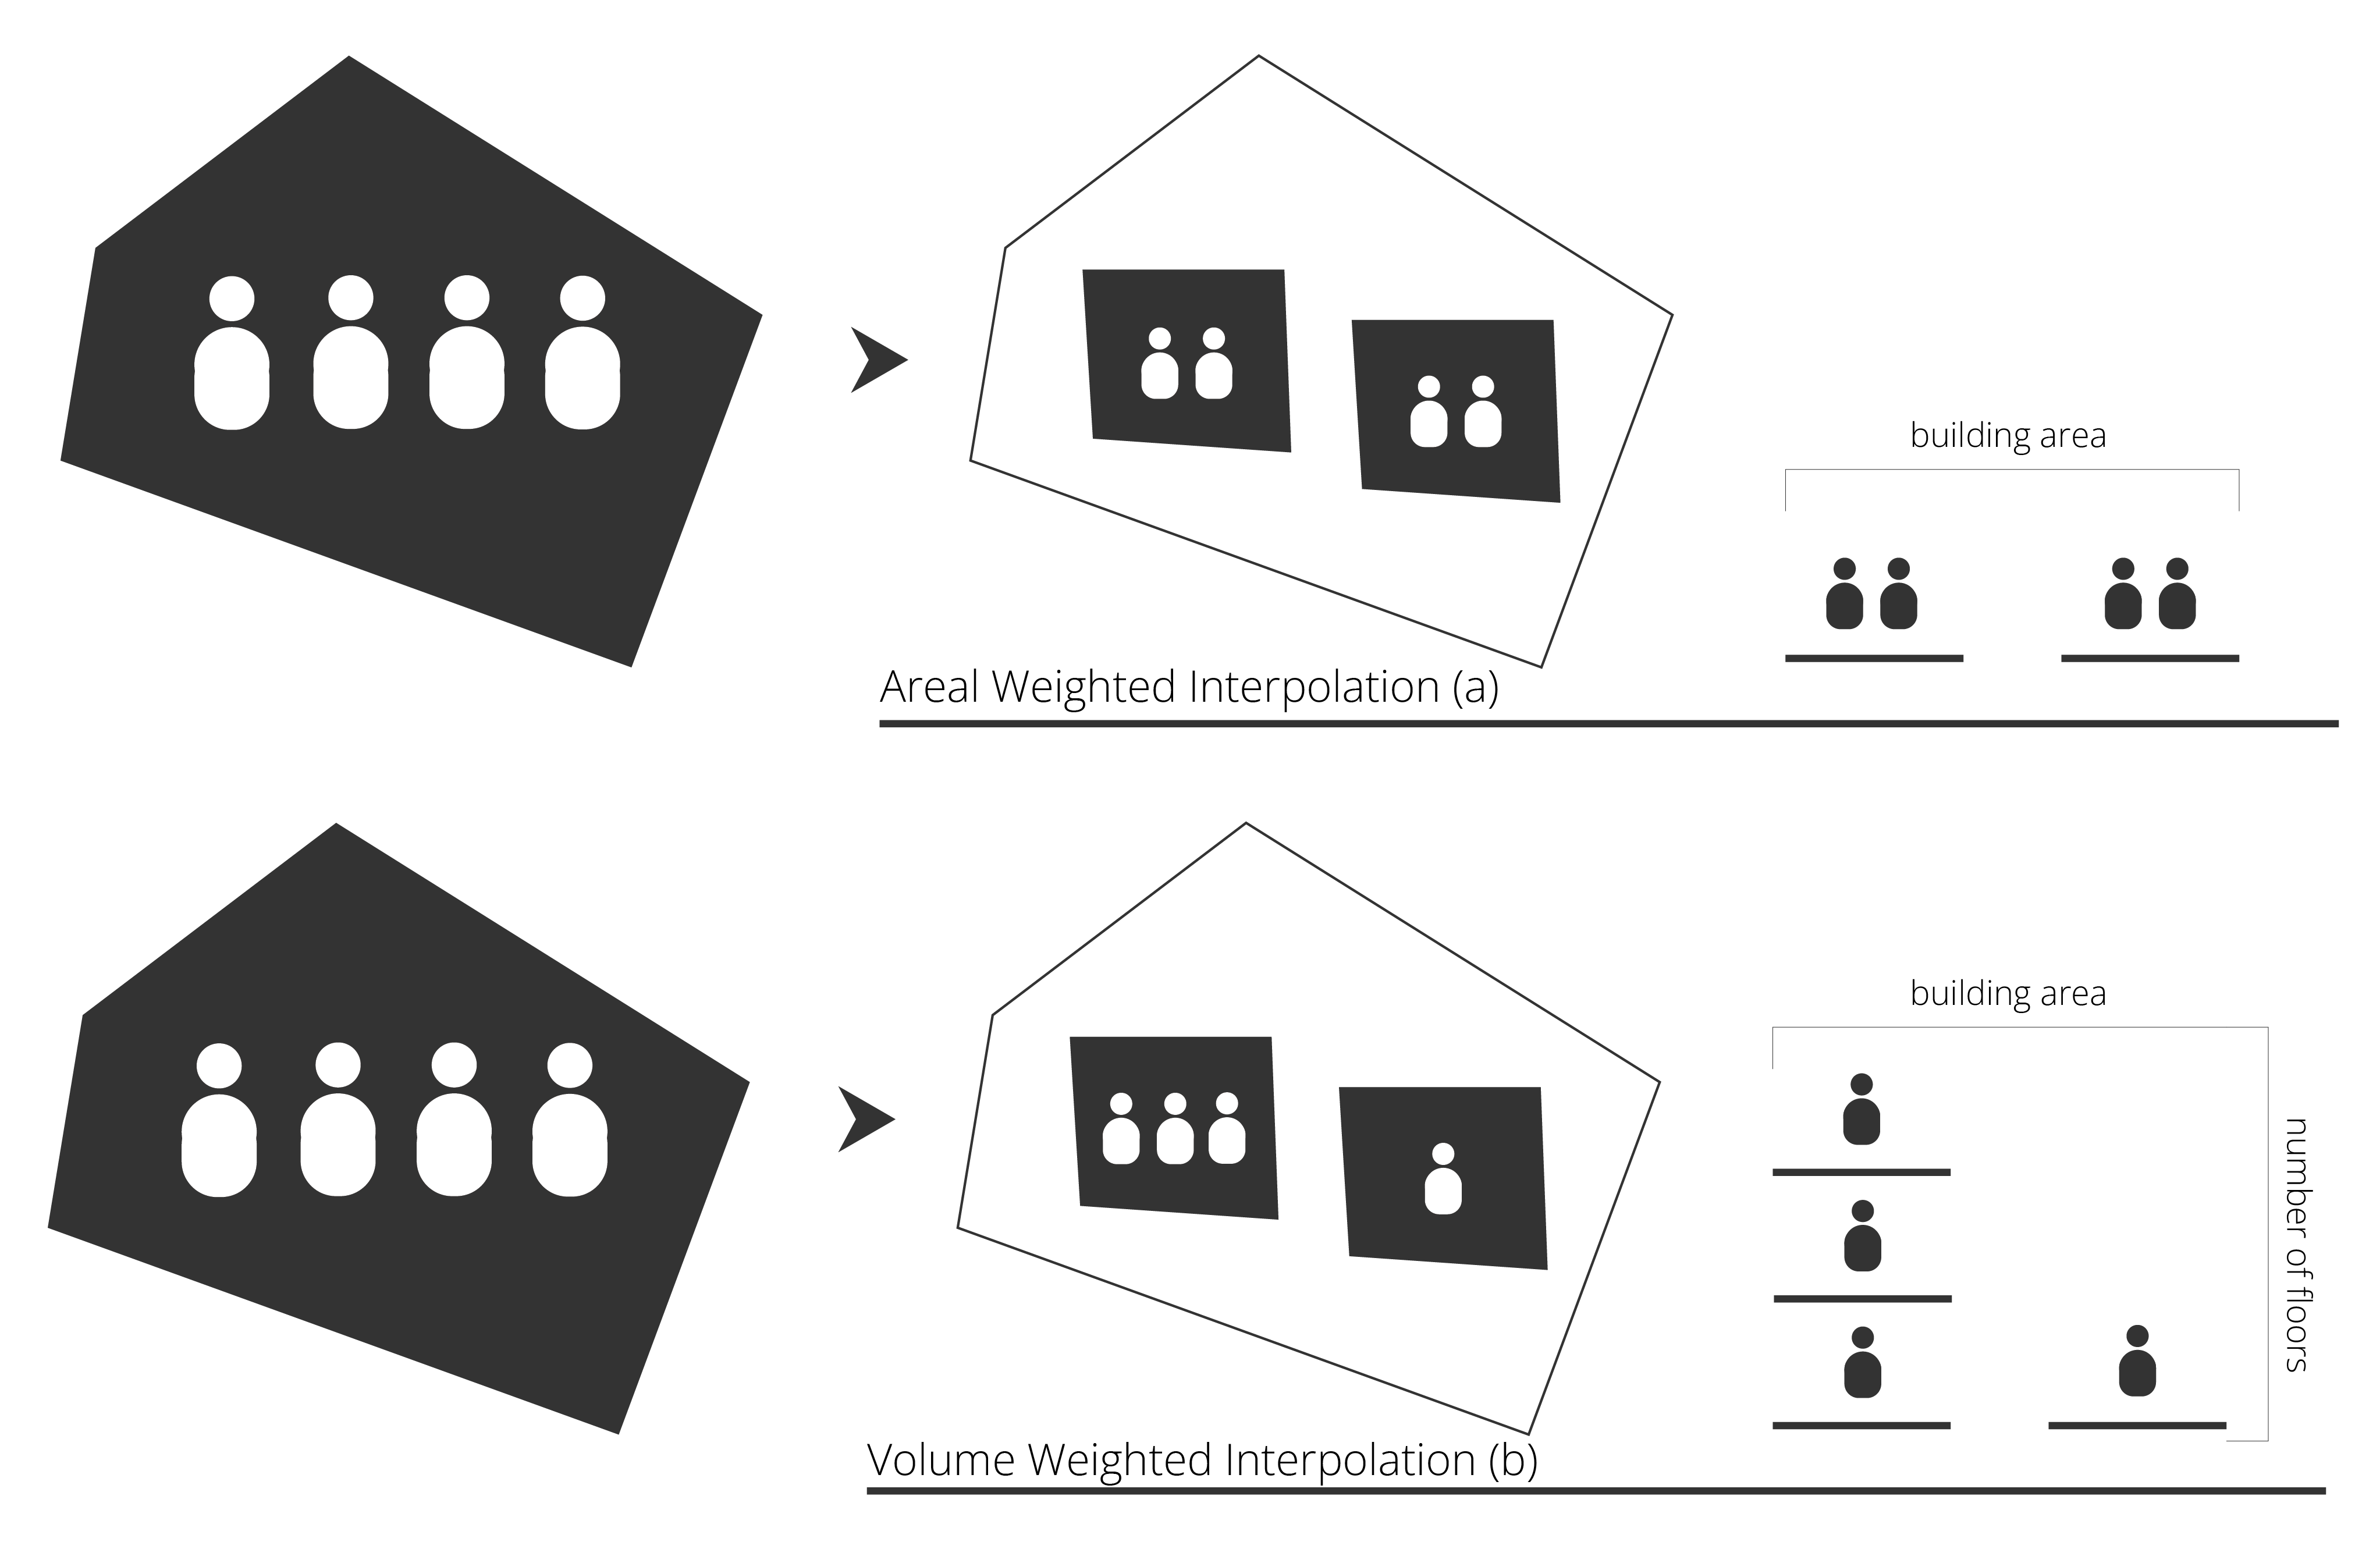
\includegraphics[width=1\linewidth]{img/methods} \caption{Illustration of the populR package's functionality. populR uses two areal interpolation methods to convert population values from city block polygons (left) to a set of individual building polygons (center). AWI (top) solely relies on the area of intersection between blocks and buildings (top-right). VWI (bottom) uses the area of intersection between blocks and buildings multiplied by the height or number of floors to aid the transformation process (bottom-right).}\label{fig:methods}
\end{figure}

\hypertarget{awi}{%
\subsubsection{AWI}\label{awi}}

\emph{AWI} proportionately interpolates the population value of the source features based on areal weights calculated by the area of intersection between the source and target zones and algebraically explained by equations \eqref{eq:eq1} and \eqref{eq:eq2} (Goodchild and Lam 1980). In equation \eqref{eq:eq1}, areal weights \(w^a_{ij}\) are calculated by standardizing the measured footprint area of individual building \(i\) in block \(j\) (\(a_{ij}\)) over the sum of building footprint areas in the \(j-th\) city block. Finally, building population values for building \(i\) in block \(j\) (\(p_{ij}\)) may be calculated by multiplying the areal weights of building \(i\) in block \(j\) with the population value of \(j-th\) block (\(P_j\)).

\begin{equation} 
  w_{ij}^a = \frac{a_{ij}}{\sum_{i=1}^{B_{j}} a_{ij}} \text{ , }
  \label{eq:eq1}
\end{equation}

\begin{equation}
    p_{ij}^a = w_{ij}^a \times P_j \text{ . }
    \label{eq:eq2}
\end{equation}

A demonstration of the \emph{AWI} approach is presented in the code block below. In the first line of code,
\CRANpkg{populR} is attached to the script. The next two lines load the package's built-in data, and the last line
demonstrates the usage of the \texttt{pp\_estimate} function. As a result, \texttt{pp\_estimate} returns an object
of class sf including individual buildings (\emph{target}) with population estimates.

\begin{verbatim}
# attach package
library(populR)

# load data
data('src')
data('trg')

# downscaling using awi
awi <- pp_estimate(target = trg, source = src, spop = pop, sid = sid,
method = awi)
\end{verbatim}

Where:

\begin{enumerate}
\def\labelenumi{\arabic{enumi}.}
\tightlist
\item
  \emph{target}: An object of class \emph{sf} that is used to interpolate data to. Usually, target may include
  polygon features representing building units
\item
  \emph{source}: An object of class \emph{sf} including data to be interpolated. Source may be a set of coarse
  polygon features, such as city blocks or census tracts
\item
  \emph{sid}: Source identification number
\item
  \emph{spop}: Source population values to be interpolated
\item
  \emph{method}: Two methods provided: \emph{AWI} (Areal Weighted Interpolation) and \emph{VWI} (Volume Weighted
  Interpolation). \emph{AWI} proportionately interpolates the population values based on areal weights
  calculated by the area of intersection between the source and target zones. \emph{VWI} proportionately
  interpolates the population values based on volume weights calculated by the area of inter-
  section between the source and target zones multiplied by the volume information (height or
  number of floors)
\end{enumerate}

\hypertarget{vwi}{%
\subsubsection{VWI}\label{vwi}}

Given the number of floors (or height) of individual buildings, \emph{VWI} applies the same logic as \emph{AWI}. Instead of areal weights, \emph{VWI} proportionately dis-aggregates source population counts using volume weights measured by the area of intersection multiplied either by individual building height (if available) or number of floors. \emph{VWI} may be mathematically expressed by equations \eqref{eq:eq3} to \eqref{eq:eq5}. First, the volume of building \(i\) in block \(j\) (\(v_{ij}\)) is measured by multiplying the footprint area (\(a_{ij}\)) of building \(i\) in block \(j\) with the number of floors or height (\(n_{ij}\)) as shown in equation \eqref{eq:eq3}. Next, volume weights (\(w^v_{ij}\)) are calculated by standardizing the volume of building \(i\) in block \(j\) (\(v_{ij}\)) by the sum of the total volume of buildings in the \(j-th\) block \eqref{eq:eq4}. Then, building population values for building \(i\) in block \(j\) (\(p^v_{ij}\)) may be calculated by multiplying the volume weights (\(w^v_{ij}\)) of building \(i\) in block \(j\) with the population value of block \(j\) (\(P_J\)) as shown in \eqref{eq:eq5}.

\begin{equation} 
    v_{ij} = a_{ij} \times n_{ij} \text{ , }
    \label{eq:eq3}
\end{equation}

\begin{equation} 
    w_{ij}^v = \frac{v_{ij}}{\sum_{i=1}^{B_{j}} v_{ij}} \text{ , }
    \label{eq:eq4}
\end{equation}

\begin{equation} 
    p_{ij}^v = w_{ij}^v \times P_j \text{ . }
    \label{eq:eq5}
\end{equation}

The code block below provides an example of the \emph{VWI} approach.

\begin{verbatim}
# downscaling using vwi
vwi <- pp_estimate(target = trg, source = src, spop = pop, sid = sid,
volume = floors, method = vwi)
\end{verbatim}

Where:

\begin{enumerate}
\def\labelenumi{\arabic{enumi}.}
\tightlist
\item
  \emph{volume}: Target feature volume information (height or number of floors). Required when method
  is set to \emph{vwi}
\end{enumerate}

It is important to mention that when volume information (number of floors or building height)
is not available for the entire target dataset, users may replace missing values with \(1\) if they want to
include them as buildings with 1 floor; otherwise, users may replace missing values with \(0\) if they
want to exclude them from the downscaling process.

\hypertarget{rounding}{%
\subsection{Rounding}\label{rounding}}

\emph{AWI} is volume-preserving (Comber and Zeng 2019) (as \emph{VWI}) and returns an object of class \emph{sf} with
decimal population counts for each target feature. To increase the readability of the results as well
as to maintain the initial source population values, it is essential for many applications to provide
integer values by rounding off to the closest integer. This transformation may result in a shortage or
surplus in comparison to the initial values (source values), and therefore, to cope with this problem,
the \texttt{pp\_round} function is proposed.

First, estimated population values are converted into integer numbers. Next, the \texttt{pp\_round} function calculates the differences between the initial population counts and the sum of the integer values for each city block; it is activated only if the quantified difference is either positive or negative. In either case, during this process, target-based differences are also calculated and used to refine the integer counts by adding or removing one population unit in order to preserve the initial source counts when summed up.

An example of the \texttt{pp\_round} function is provided below.

\begin{verbatim}
# downscaling using awi
awi <- pp_round(x = awi, tpop = pp_est, spop = pop, sid = sid)

# downscaling using awi
vwi <- pp_round(x = vwi, tpop = pp_est, spop = pop, sid = sid)
\end{verbatim}

Where:

\begin{enumerate}
\def\labelenumi{\arabic{enumi}.}
\tightlist
\item
  \emph{x}: An object of class sf obtained by the \texttt{pp\_estimate} function
\item
  \emph{tpop}: Target population estimates obtained by the \texttt{pp\_estimate} function
\item
  \emph{spop}: Initial source population values (included after the implementation of the \texttt{pp\_estimate}
  function)
\item
  \emph{sid}: Source identification number
\end{enumerate}

As a result, \texttt{pp\_round} returns an object of class \emph{sf} with integer estimates of population values
with respect to the initial source population values.

\hypertarget{comparing}{%
\subsection{Comparing}\label{comparing}}

Volume-preserving means that estimated values should sum up to the initial population counts for each source unit, and therefore, one may need to compare target estimates to the initial source values. For this purpose, a function is introduced under the alias \texttt{pp\_compare}. The \texttt{pp\_compare} function measures the root mean squared error (RMSE), the mean absolute error (MAE), and finally, the statistical relationship between the initial source values and the estimated ones, which is calculated and depicted on a 2D scatter diagram along with the value of the correlation coefficient \(R^2\).

A short example of the \texttt{pp\_compare} function is presented in the code block below, where \emph{src\_awi} (and \emph{src\_vwi}) is a \emph{data.frame} created by grouping the sum of the estimated values along with the initial population values for each source feature.

\begin{verbatim}
# attach library
library(dplyr)

# group estimated and actual values by source identification number - awi
src_awi <- awi %>%
  group_by(sid) %>%
  summarise(est = sum(pp_est), act = unique(pop))

# awi approach compare to source values
pp_compare(x = src_awi, estimated = est, actual = act, title = "awi vs source")

# group estimated and actual values by source identification number - vwi
src_vwi <- vwi %>%
  group_by(sid) %>%
  summarise(est = sum(pp_est), act = unique(pop))

# vwi approach compare to source values
pp_compare(x = src_vwi, estimated = est, actual = act, title = "vwi vs source")
\end{verbatim}

Where:

\begin{enumerate}
\def\labelenumi{\arabic{enumi}.}
\tightlist
\item
  \emph{x}: An object of class \emph{sf} or a \emph{data.frame} including estimated and actual values
\item
  \emph{estimated}: Target population estimates obtained by the \texttt{pp\_estimate} function
\item
  \emph{actual}: Actual population values
\item
  \emph{title}: Scatterplot title (quoted)
\end{enumerate}

\texttt{pp\_compare} returns a list of elements with RMSE, MAE, linear regression, and \(R^2\) coefficient
information.

\hypertarget{numerical-experimentation}{%
\section{Numerical Experimentation}\label{numerical-experimentation}}

In this section, the results of the \CRANpkg{populR} package are illustrated and further compared to \CRANpkg{sf} and \CRANpkg{areal}. The analysis focus on implementation, comparison to a reference data set, and performance.

\hypertarget{case-study}{%
\subsection{Case study}\label{case-study}}

To examine the efficacy and efficiency of the \CRANpkg{populR} extension based on actual data, a small part of
the city of Mytilini was chosen as the subject for a case study (Figure \ref{fig:studyarea}). The study area consists of 9
city blocks (\emph{src}), 179 buildings (\emph{trg}), and 911 residents.

\begin{figure}
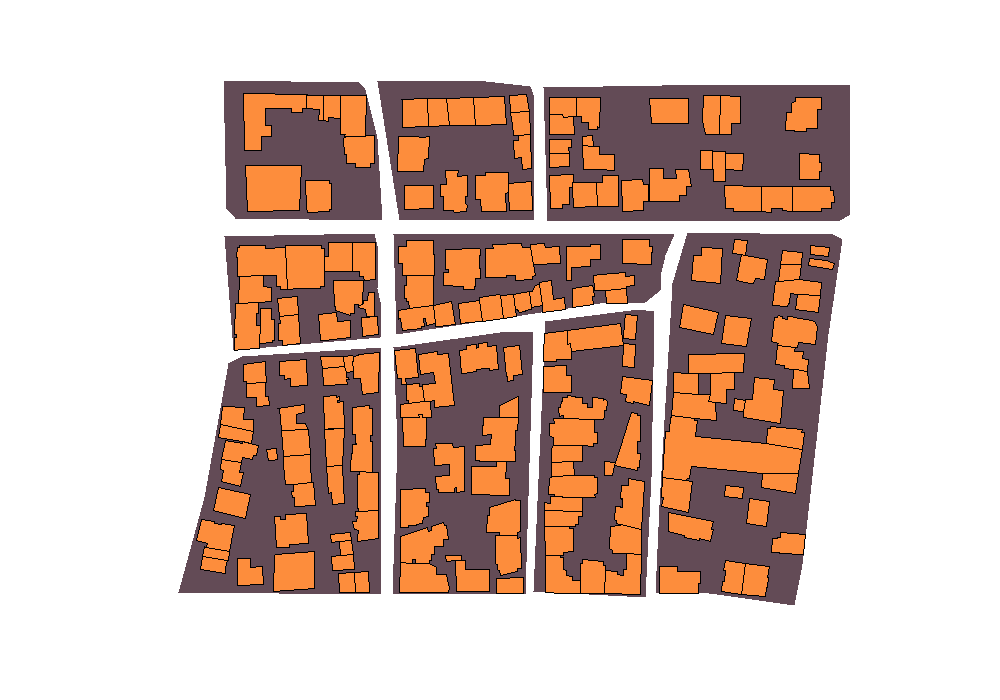
\includegraphics[width=1\linewidth]{img/study_area} \caption{Part of the city of Mytilini used as the case study for numerical experiments. The study area is represented by 9 city blocks and 179 buildings (in orange). The study area counts 911 residents.}\label{fig:studyarea}
\end{figure}

\begin{table}

\caption{\label{tab:dtbl-ltx}Data used for numerical experiments}
\centering
\fontsize{7}{9}\selectfont
\begin{tabular}[t]{l|l|l|l}
\hline
Title & Format & Source & Year\\
\hline
City block population counts & Tabular & Hellenic Statistical Authority & 2011\\
\hline
City blocks & Spatial & Hellenic Statistical Authority & 2011\\
\hline
Buildings & Spatial & Hellenic Statistical Authority & 2011\\
\hline
\end{tabular}
\end{table}

Table \ref{tab:dtbl-ltx} presents the data used in this case study. City block population counts were retrieved in tabular format while city blocks (source - \emph{src}) and buildings (target - \emph{trg}) were provided in spatial format. City block population counts and city blocks and buildings correspond to the 2011 Census of Housing and Population (Hellenic Statistical Authority 2014).

\hypertarget{implementation}{%
\subsection{Implementation}\label{implementation}}

In this section, a demonstration of the \CRANpkg{sf}, \CRANpkg{areal} and \CRANpkg{populR} packages takes place. First, the packages are attached to the script and next, \CRANpkg{populR} built-in data are loaded. Then, areal interpolation
implementation follows for each one of the aforementioned packages.

For the reader's convenience, names were shortened as follows: a) \emph{awi}: \CRANpkg{populR} \emph{AWI} approach, b)
\emph{VWI}: \CRANpkg{populR} \emph{vwi} approach, c) \emph{aws}: \CRANpkg{areal} using extensive interpolation and \emph{sum weights}, d) \emph{awt}: \CRANpkg{areal} using extensive interpolation and \emph{total weights}, and e) \emph{sf}: \CRANpkg{sf} using extensive interpolation and \emph{total weights}.

\begin{verbatim}
# attach libraries
library(populR)
library(areal)
library(sf)

# load data
data("trg", package = "populR")
data("src", package = "populR")

# populR - awi
awi <- pp_estimate(target = trg, source = src, spop = pop, sid = sid,
method = awi)

# populR - vwi
vwi <- pp_estimate(target = trg, source = src, spop = pop, sid = sid,
volume = floors, method = vwi)

# areal - sum weights
aws <- aw_interpolate(trg, tid = tid, source = src, sid = 'sid',
weight = 'sum', output = 'sf', extensive = 'pop')

# areal - total weights
awt <- aw_interpolate(trg, tid = tid, source = src, sid = 'sid',
weight = 'total', output = 'sf', extensive = 'pop')

# sf - total weights
sf <- st_interpolate_aw(src['pop'], trg, extensive = TRUE)
\end{verbatim}

Evidently, \CRANpkg{sf} requires less arguments than \CRANpkg{populR} and \CRANpkg{areal}, which makes it very easy to implement. \CRANpkg{populR} requires at least 5 arguments, and \CRANpkg{areal} at least 7, which may increase the implementation complexity.

The study area counts 911 residents, as already mentioned in previous section. \emph{awi}, \emph{vwi} and \emph{aws}
correctly estimated population values as they sum to 911, while \emph{awt} and \emph{sf} underestimated values.
This is expected as both methods use the total area of the source features during the interpolation
process and are useful when source and target features completely overlap.

Moreover, identical results were obtained by the \emph{awi} and \emph{aws} approaches, but somehow different
results were obtained by the \emph{vwi}, as shown in Table \ref{tab:rtbl-ltx}.

\begin{table}

\caption{\label{tab:rtbl-ltx}Implementation results obtained by awi, vwi, awt, aws and sf for 10 buildings of the study area.}
\centering
\fontsize{7}{9}\selectfont
\begin{tabular}[t]{r|r|r|r|r|r}
\hline
nr & awi & vwi & aws & awt & sf\\
\hline
1 & 1.36 & 0.37 & 1.36 & 0.58 & 0.58\\
\hline
2 & 1.42 & 0.39 & 1.42 & 0.60 & 0.60\\
\hline
3 & 16.12 & 15.47 & 16.12 & 5.99 & 5.99\\
\hline
4 & 7.47 & 4.30 & 7.47 & 2.77 & 2.77\\
\hline
5 & 2.22 & 0.61 & 2.22 & 0.94 & 0.94\\
\hline
6 & 21.08 & 28.32 & 21.08 & 7.83 & 7.83\\
\hline
7 & 1.34 & 0.44 & 1.34 & 0.62 & 0.62\\
\hline
8 & 2.57 & 1.45 & 2.57 & 1.36 & 1.36\\
\hline
9 & 6.54 & 5.03 & 6.54 & 2.75 & 2.75\\
\hline
10 & 6.68 & 3.84 & 6.68 & 2.48 & 2.48\\
\hline
\end{tabular}
\end{table}

Finally, visual representations of the results are shown in Figure \ref{fig:maps}.

\begin{figure}
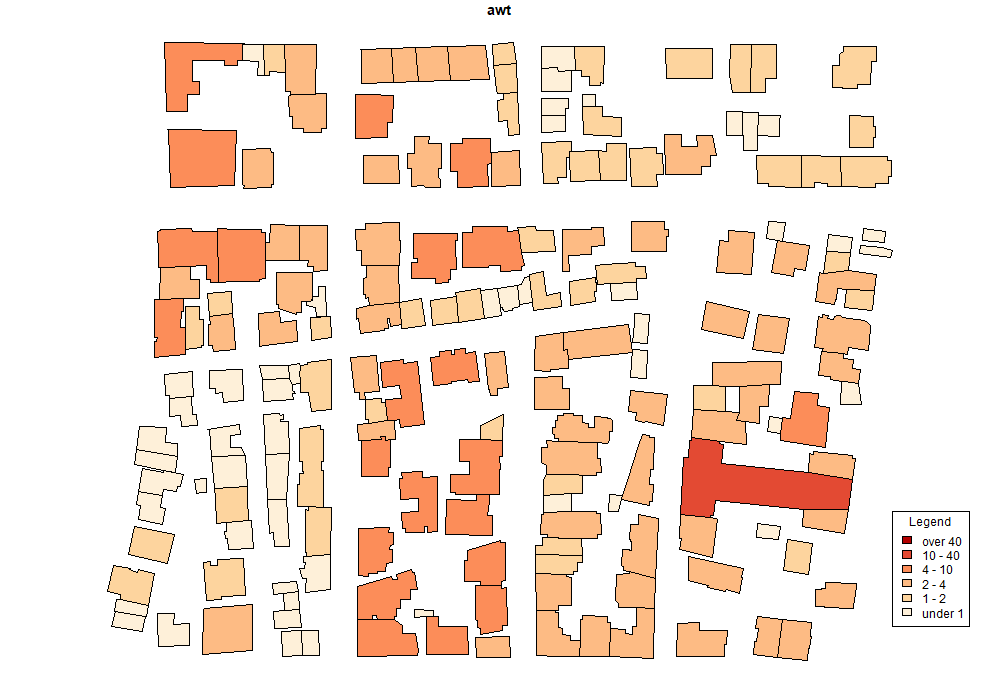
\includegraphics[width=0.49\linewidth,height=0.2\textheight]{img/result_maps/map_awt} 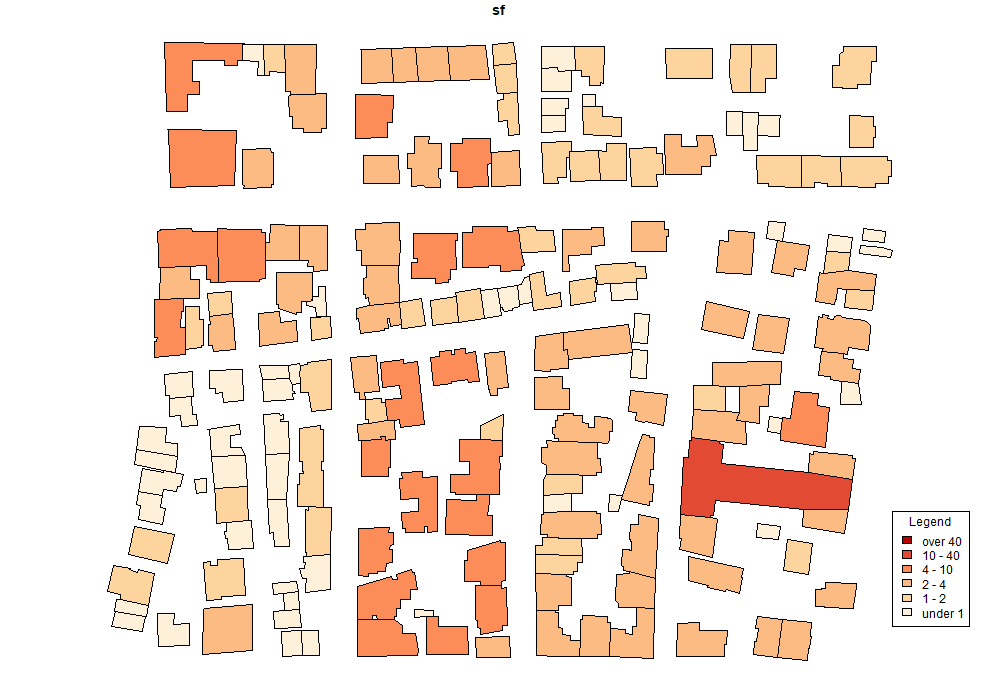
\includegraphics[width=0.49\linewidth,height=0.2\textheight]{img/result_maps/map_sf} 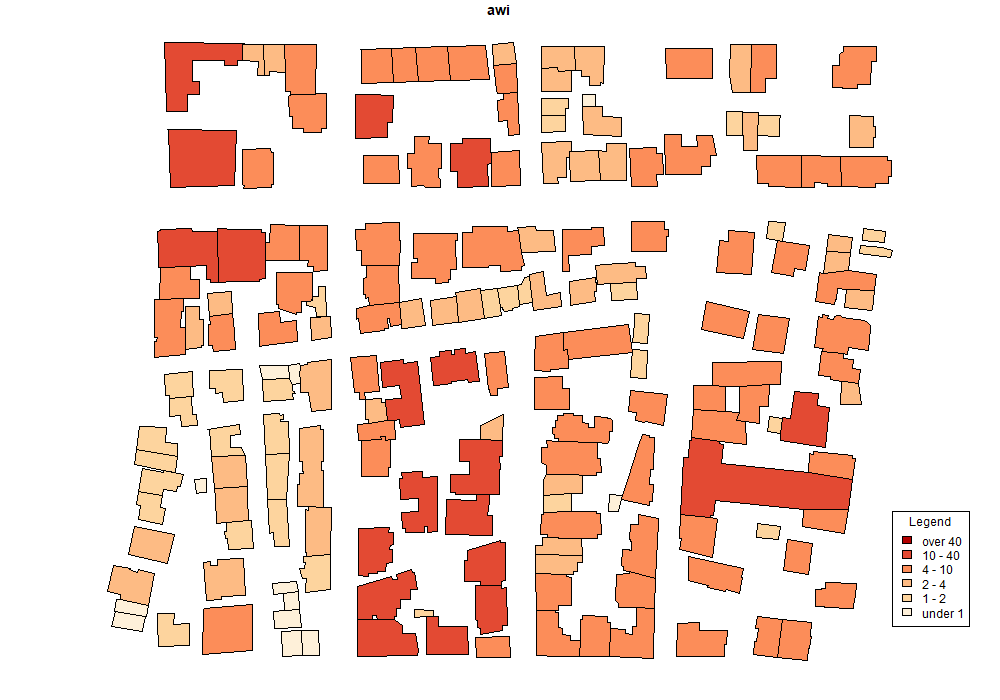
\includegraphics[width=0.49\linewidth,height=0.2\textheight]{img/result_maps/map_awi} 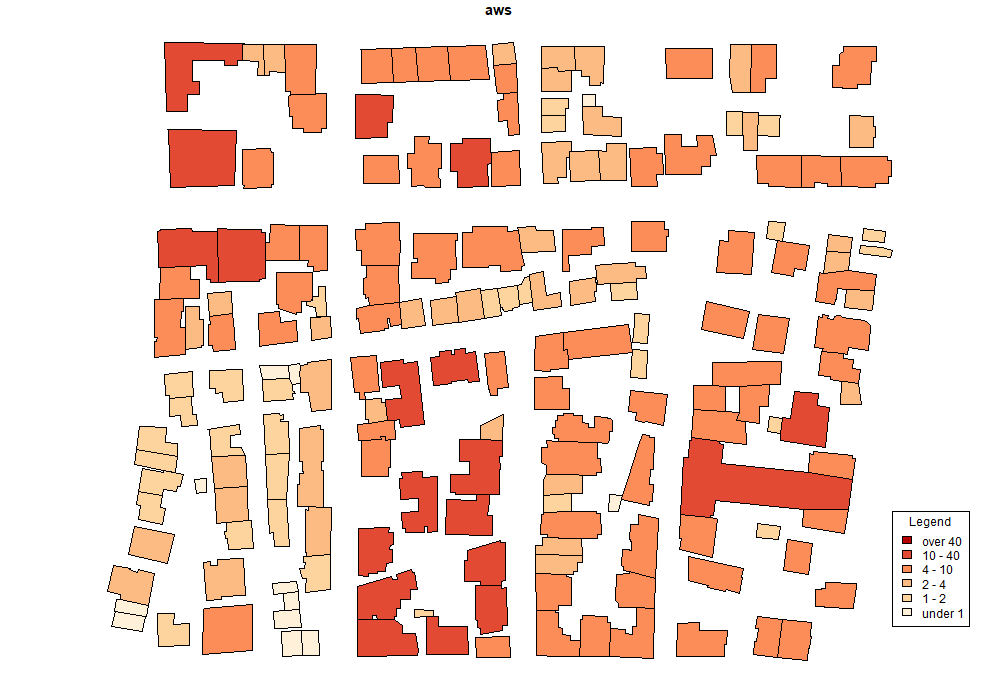
\includegraphics[width=0.49\linewidth,height=0.2\textheight]{img/result_maps/map_aws} 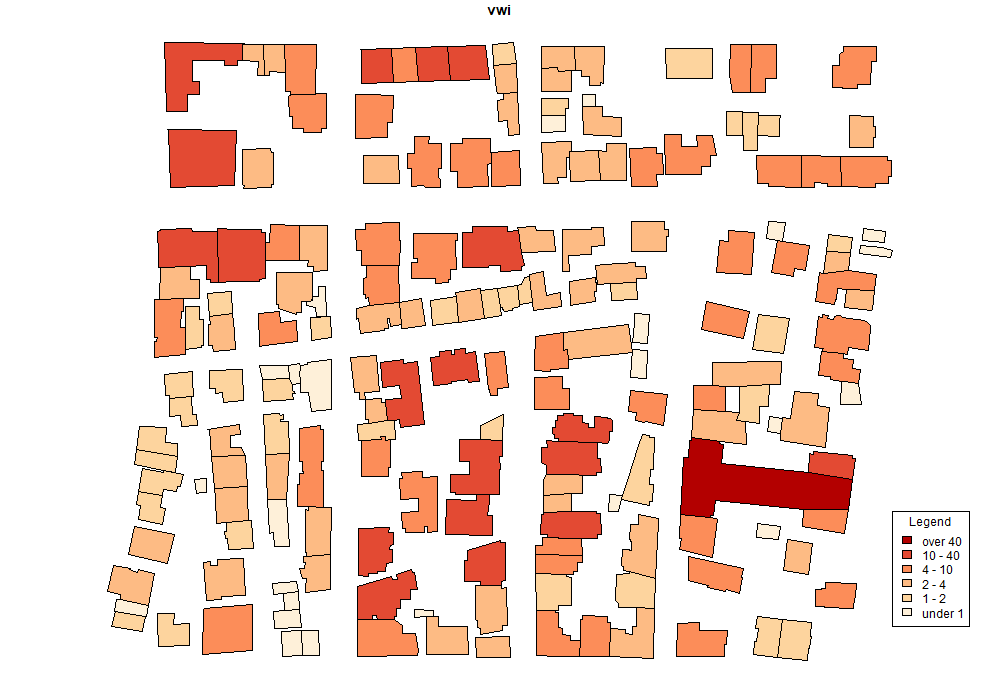
\includegraphics[width=0.49\linewidth,height=0.2\textheight]{img/result_maps/map_vwi} \caption{Cartographic representation of the downscaling results acquired by a) awt (top-left), b) sf (top-right), c) awi (center-left), d) aws (center-right), and e) vwi (bottom). awt and sf use the same formula therefore, they provide similar results. Additionally, the same results obtained by aws and awi as they are based on the same formula. vwi provide somehow different distribution because of the influence of the volume weights during the interpolation process.}\label{fig:maps}
\end{figure}

\hypertarget{comparison-to-reference-data}{%
\subsection{Comparison to reference data}\label{comparison-to-reference-data}}

Due to confidentiality concerns, population data at the granularity of building are not publicly available in Greece. Therefore, an alternate population distribution previously published in Batsaris et al. (2019) was used as reference data (\emph{rf}). \emph{rf} population values are also included in the build-in \emph{trg} data set.

Using the \texttt{pp\_compare} function as shown in the example below, we investigated the statistical relationship between \emph{rf} and the results obtained by \CRANpkg{populR}, \CRANpkg{areal}, and \CRANpkg{sf} packages.

\begin{verbatim}
# compare awi to rf
pp_compare(data, estimated = awi, actual = rf, title = "awi vs rf")

# compare vwi to rf
pp_compare(data, estimated = vwi, actual = rf, title = "vwi vs rf")

# compare sf to rf
pp_compare(data, estimated = sf, actual = rf, title = "sf vs rf")

# compare awt to rf
pp_compare(data, estimated = awt, actual = rf, title = "awt vs rf")

# compare aws to rf
pp_compare(data, estimated = aws, actual = rf, title = "aws vs rf")
\end{verbatim}

Table \ref{tab:2rtbl-ltx} presents the results obtained for the first 10 individual buildings for each implementation in comparison to \emph{rf} values. Additionally, \(RMSE\), \(MAE\), and \(R^2\) values are measured and depicted in
Table \ref{tab:ertbl-ltx} and finally, scatter diagrams provided in Figure \ref{fig:scatterplots}.

Generally the scatter diagrams (Figure \ref{fig:scatterplots-ltx})) suggest strong and positive relationships in all cases. However, the \emph{vwi} approach obtained the best results and achieved the smallest \(RMSE\) (1.44824) and \(MAE\) (0.9358159) values and the largest \(R^2\) (0.9878) value as shown in Table and Figure. Moreover, \emph{aws} and \emph{awi} provided the same error and \(R^2\) measurements (\(RMSE\): 5.325914, \(MAE\): 2.748126 and \(R^2\): 0.8215). \emph{sf} and \emph{awt} provided the same results and performed poorly in comparison to \emph{vwi} by obtaining the largest error measurements and the smallest \(R^2\) (\(RMSE\): 7.416329, \(MAE\): 3.664695, and \(R^2\): 0.80367).

\begin{table}

\caption{\label{tab:2rtbl-ltx}Implementation results obtained by awi, vwi, awt, aws and sf for 10 buildings of the study area in comparison to reference data (rf).}
\centering
\fontsize{7}{9}\selectfont
\begin{tabular}[t]{r|r|r|r|r|r|r}
\hline
nr & rf & awi & vwi & aws & awt & sf\\
\hline
1 & 0.46 & 1.36 & 0.37 & 1.36 & 0.58 & 0.58\\
\hline
2 & 0.49 & 1.42 & 0.39 & 1.42 & 0.60 & 0.60\\
\hline
3 & 16.20 & 16.12 & 15.47 & 16.12 & 5.99 & 5.99\\
\hline
4 & 5.63 & 7.47 & 4.30 & 7.47 & 2.77 & 2.77\\
\hline
5 & 0.76 & 2.22 & 0.61 & 2.22 & 0.94 & 0.94\\
\hline
6 & 31.77 & 21.08 & 28.32 & 21.08 & 7.83 & 7.83\\
\hline
7 & 0.49 & 1.34 & 0.44 & 1.34 & 0.62 & 0.62\\
\hline
8 & 1.57 & 2.57 & 1.45 & 2.57 & 1.36 & 1.36\\
\hline
9 & 3.75 & 6.54 & 5.03 & 6.54 & 2.75 & 2.75\\
\hline
10 & 5.03 & 6.68 & 3.84 & 6.68 & 2.48 & 2.48\\
\hline
\end{tabular}
\end{table}

\begin{table}

\caption{\label{tab:ertbl-ltx}RMSE, MAE and R\textsuperscript{2} values were calculated to assess the estimation accuracy using rf as the control variable. vwi provide the best measurements.}
\centering
\fontsize{7}{9}\selectfont
\begin{tabular}[t]{l|r|r|r}
\hline
Title & RMSE & MAE & R\textsuperscript{2}\\
\hline
rf vs vwi & 1.45 & 0.94 & 0.988\\
\hline
rf vs awi & 5.33 & 2.75 & 0.822\\
\hline
rf vs aws & 5.33 & 2.75 & 0.822\\
\hline
rf vs sf & 7.42 & 3.66 & 0.804\\
\hline
rf vs awt & 7.42 & 3.66 & 0.804\\
\hline
\end{tabular}
\end{table}

\begin{figure}
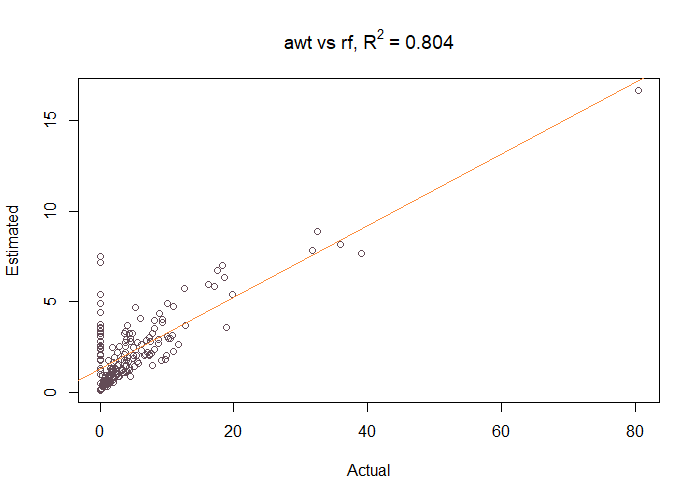
\includegraphics[width=0.49\linewidth]{img/result_figs/rf_vs_awt} 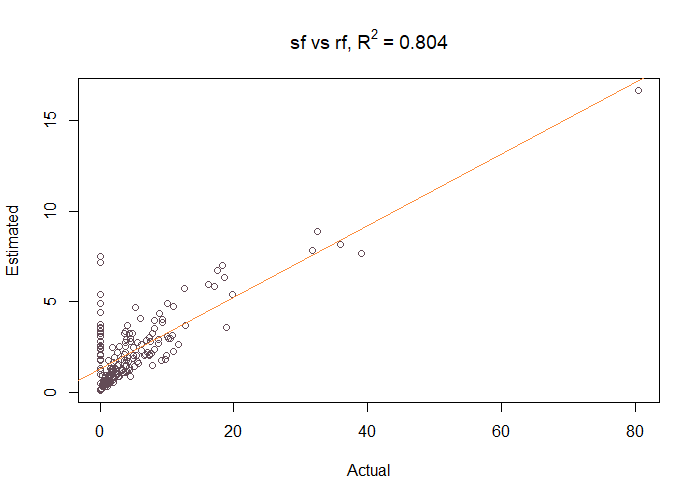
\includegraphics[width=0.49\linewidth]{img/result_figs/rf_vs_sf} 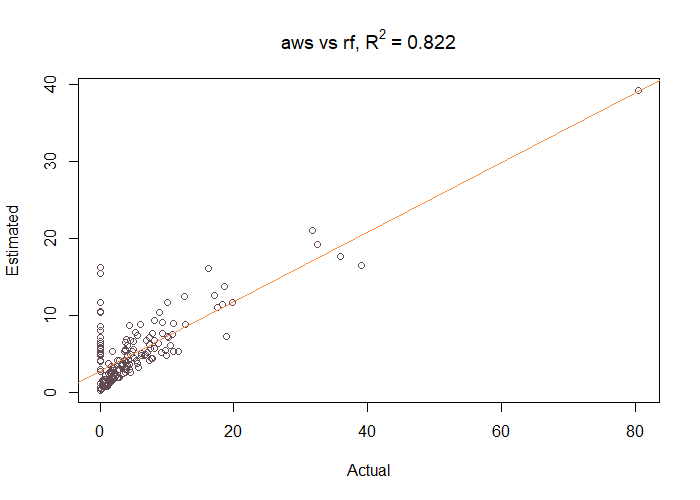
\includegraphics[width=0.49\linewidth]{img/result_figs/rf_vs_aws} 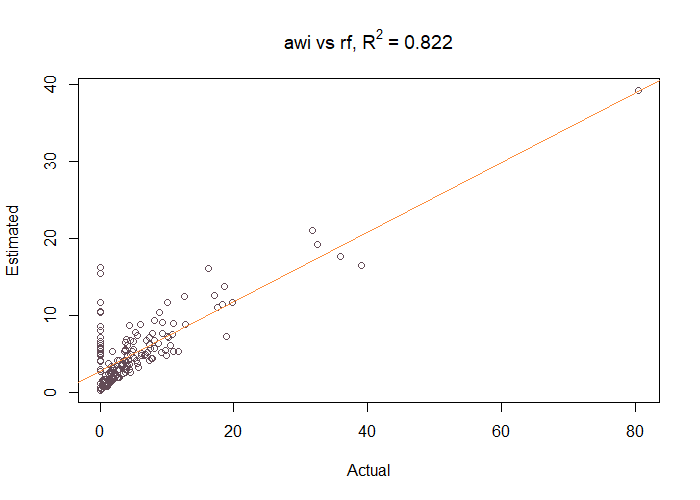
\includegraphics[width=0.49\linewidth]{img/result_figs/rf_vs_awi} 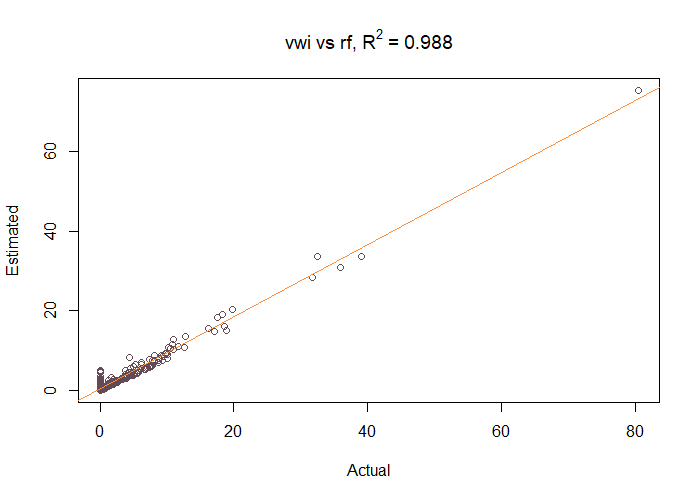
\includegraphics[width=0.49\linewidth]{img/result_figs/rf_vs_vwi} \caption{Investigation of the relationship of the outcomes and reference data (rf) as the control variable. a) rf vs awt, R\textsuperscript{2} = 0.804 (top-left), b) rf vs sf, R\textsuperscript{2} = 0.804 (top-right), c) rf vs aws, R\textsuperscript{2} = 0.822 (center-left), d) rf vs awi, R\textsuperscript{2} = 0.822 (center-right) and e) rf vs vwi, R\textsuperscript{2} = 0.988.}\label{fig:scatterplots-ltx}
\end{figure}

\hypertarget{performance}{%
\subsection{Performance}\label{performance}}

In this section, a performance comparison (execution times) takes place using the \CRANpkg{microbenchmark}
package. Performance tests are carried out using the sample data provided by \CRANpkg{populR} as well as
external data sets from a significantly larger study area (Chios, Greece) with 845 city blocks and 15,946
buildings.

Execution time measurements for both cases are shown in Tables \ref{tab:bidp-ltx} and \ref{tab:chdp-ltx} accordingly. In both
cases, execution time measurements suggest that \CRANpkg{populR} performs faster than \CRANpkg{areal} and \CRANpkg{sf}. Using the built-in data, \emph{awi} and \emph{vwi} scored the best mean execution time (about 76 milliseconds), which is about
54 millisecond faster than \emph{aws}, 61 milliseconds faster than \emph{sf}, and almost 70 milliseconds faster than
\emph{awt.}

\begin{table}

\caption{\label{tab:bidp-ltx}Execution time measurement comparisons (in milliseconds) using microbenchmark and sample data}
\centering
\fontsize{7}{9}\selectfont
\begin{tabular}[t]{l|r|r|r}
\hline
Name & Min & Mean & Max\\
\hline
vwi & 74.06 & 76.23 & 84.39\\
\hline
awi & 74.31 & 75.91 & 99.70\\
\hline
aws & 128.48 & 132.56 & 143.97\\
\hline
awt & 172.08 & 176.27 & 185.86\\
\hline
sf & 136.48 & 142.33 & 289.38\\
\hline
\end{tabular}
\end{table}

\begin{table}

\caption{\label{tab:chdp-ltx}Execution time measurement comparisons (in seconds) using microbenchmark and external
data}
\centering
\fontsize{7}{9}\selectfont
\begin{tabular}[t]{l|r|r|r}
\hline
Name & Min & Mean & Max\\
\hline
vwi & 1.55 & 1.67 & 1.94\\
\hline
awi & 1.55 & 1.68 & 1.95\\
\hline
aws & 2.26 & 2.39 & 2.64\\
\hline
awt & 2.27 & 2.42 & 2.62\\
\hline
sf & 2.63 & 2.79 & 3.17\\
\hline
\end{tabular}
\end{table}

\hypertarget{conclusions}{%
\section{Conclusions}\label{conclusions}}

This study is an attempt to contribute to the continuously growing scientific literature of population
downscaling using areal interpolation methods. Despite the fact that there are so many downscaling
methods developed, only a few implementation tools are available to the GIS and R community, and
therefore, it may be challenging for non-expert GIS users to take advantage of these methods (Mennis 2009; Langford 2007). Due to this lack of implementation tools, this study attempts to fill this gap
by introducing \CRANpkg{populR}, an R package for population downscaling using areal interpolation methods.

This package implements two areal interpolation methods, namely \emph{awi} and \emph{vwi.} The \emph{awi} approach
guides the interpolation process using the area of intersection between source and target zones while
\emph{vwi} uses the number of floors as additional information to influence the downscaling process. The
package is available to the R community though the CRAN and Github repositories.

In order to show the efficacy and efficiency of the introduced package on actual data, a subset
area of the city of Mytilini, Greece, was used in the case study. Moreover, a comparative analysis
between \CRANpkg{populR}, \CRANpkg{areal}, and \CRANpkg{sf} was carried out, and the results showed that \emph{vwi} outperformed others by achieving the smallest error measurements, easy implementation and faster execution times. Thus,
we strongly believe that R users will gain significant advantage by using \CRANpkg{populR} for population
downscaling.

The evaluation of the results indicates the potential of \CRANpkg{populR} in providing better and faster results
in comparison to existing R packages. However, we believe that the results may be further improved
by incorporating new forms of data, such as Volunteered Geographic Information (VGI), acquired
from either social media or open spatial databases such as Open Street Map (Bakillah et al. 2014; Guo, Cao, and Wang 2017; Yang et al. 2019; Comber and Zeng 2019). By incorporating VGI as ancillary information, we can identify different types of buildings and therefore adjust the weight calculation accordingly. This will be an important improvement that would be helpful for R users interested in population
downscaling.

\hypertarget{references}{%
\section*{References}\label{references}}
\addcontentsline{toc}{section}{References}

\hypertarget{refs}{}
\begin{CSLReferences}{1}{0}
\leavevmode\vadjust pre{\hypertarget{ref-Ahola2007}{}}%
Ahola, Terhi, Kirsi Virrantaus, Jukka Matthias Krisp, and Gary J. Hunter. 2007. {``A Spatio-Temporal Population Model to Support Risk Assessment and Damage Analysis for Decision-Making.''} \emph{International Journal of Geographical Information Science} 21 (8): 935--53. \url{https://doi.org/10.1080/13658810701349078}.

\leavevmode\vadjust pre{\hypertarget{ref-Bahadori2021}{}}%
Bahadori, Mohammad Sadegh, Alexandre B. Gonçalves, and Filipe Moura. 2021. {``A Systematic Review of Station Location Techniques for Bicycle-Sharing Systems Planning and Operation.''} \emph{ISPRS International Journal of Geo-Information} 10 (8): 554. \url{https://doi.org/10.3390/ijgi10080554}.

\leavevmode\vadjust pre{\hypertarget{ref-Bakillah2014}{}}%
Bakillah, Mohamed, Steve Liang, Amin Mobasheri, Jamal Jokar Arsanjani, and Alexander Zipf. 2014. {``Fine-Resolution Population Mapping Using OpenStreetMap Points-of-Interest.''} \emph{International Journal of Geographical Information Science} 28 (9): 1940--63. \url{https://doi.org/10.1080/13658816.2014.909045}.

\leavevmode\vadjust pre{\hypertarget{ref-populr}{}}%
Batsaris, Marios. 2022. \emph{{populR}: Population Downscaling}. \url{https://CRAN.R-project.org/package=populR}.

\leavevmode\vadjust pre{\hypertarget{ref-Batsaris2019}{}}%
Batsaris, Marios, Dimitris Kavroudakis, Nikolaos A. Soulakellis, and Themistoklis Kontos. 2019. {``Location-Allocation Modeling for Emergency Evacuation Planning in a Smart City Context.''} \emph{International Journal of Applied Geospatial Research} 10 (4): 28--43. \url{https://doi.org/10.4018/ijagr.2019100103}.

\leavevmode\vadjust pre{\hypertarget{ref-Bian2015}{}}%
Bian, Ruijie, and Chester G. Wilmot. 2015. {``Spatiotemporal Population Distribution Method for Emergency Evacuation.''} \emph{Transportation Research Record: Journal of the Transportation Research Board} 2532 (1): 99--106. \url{https://doi.org/10.3141/2532-12}.

\leavevmode\vadjust pre{\hypertarget{ref-Calka2017}{}}%
Calka, Beata, Joanna Nowak Da Costa, and Elzbieta Bielecka. 2017. {``Fine Scale Population Density Data and Its Application in Risk Assessment.''} \emph{Geomatics, Natural Hazards and Risk} 8 (2): 1440--55. \url{https://doi.org/10.1080/19475705.2017.1345792}.

\leavevmode\vadjust pre{\hypertarget{ref-Comber2019}{}}%
Comber, Alexis, and Wen Zeng. 2019. {``Spatial Interpolation Using Areal Features: A Review of Methods and Opportunities Using New Forms of Data with Coded Illustrations.''} \emph{Geography Compass} 13 (10): 1--23. \url{https://doi.org/10.1111/gec3.12465}.

\leavevmode\vadjust pre{\hypertarget{ref-Dobson2000}{}}%
Dobson, J E, E A Bright, R G Durfee, and B A Worley. 2000. {``LandScan: A Global Population Database for Estimating Population at Risk.''} \emph{Photogrammetric Engineering and Remote Sensing} 66 (7): 849--57.

\leavevmode\vadjust pre{\hypertarget{ref-EU2009}{}}%
European Union, EU. 2009. {``European Parliament and Council Regulation (EC) No 763/2008 on Population and Housing Censuses.''} \url{https://ec.europa.eu/eurostat/web/population-demography/population-housing-censuses/legislation}.

\leavevmode\vadjust pre{\hypertarget{ref-Fisher1995}{}}%
Fisher, F. Peter, and Mitchel Langford. 1995. {``Modelling the Errors in Areal Interpolation Between Zonal Systems by Monte Carlo Simulation.''} \emph{Environment and Planning A} 27: 211--24. \url{https://doi.org/10.1068/a270211}.

\leavevmode\vadjust pre{\hypertarget{ref-Freire2012}{}}%
Freire, S., and C. Aubrecht. 2012. {``Integrating Population Dynamics into Mapping Human Exposure to Seismic Hazard.''} \emph{Natural Hazards and Earth System Science} 12 (11): 3533--43. \url{https://doi.org/10.5194/nhess-12-3533-2012}.

\leavevmode\vadjust pre{\hypertarget{ref-Goodchild1980}{}}%
Goodchild, Michael F., and Siu-Ngan Nina Lam. 1980. {``Areal Interpolation: A Variant of the Traditional Spatial Problem.''} \emph{Geo-Processing} 1 (3): 297--312.

\leavevmode\vadjust pre{\hypertarget{ref-Guo2017}{}}%
Guo, Hui, Kai Cao, and Peng Wang. 2017. {``Population Estimation in Singapore Based on Remote Sensing and Open Data.''} \emph{International Archives of the Photogrammetry, Remote Sensing and Spatial Information Sciences - ISPRS Archives} 42: 1181--87. \url{https://doi.org/10.5194/isprs-archives-XLII-2-W7-1181-2017}.

\leavevmode\vadjust pre{\hypertarget{ref-Han2020}{}}%
Han, Bing, Mingxing Hu, and Jialing Wang. 2020. {``Site Selection for Pre-Hospital Emergency Stations Based on the Actual Spatiotemporal Demand: A Case Study of Nanjing City, China.''} \emph{ISPRS International Journal of Geo-Information} 9 (10): 542. \url{https://doi.org/10.3390/ijgi9100559}.

\leavevmode\vadjust pre{\hypertarget{ref-HSA2014}{}}%
Hellenic Statistical Authority, HSA. 2014. {``2011 Population and Housing Census of Greece.''} Hellenic Statistical Authority.

\leavevmode\vadjust pre{\hypertarget{ref-Kim2010}{}}%
Kim, Hwahwan, and Xiaobai Yao. 2010. {``Pycnophylactic Interpolation Revisited: Integration with the Dasymetric-Mapping Method.''} \emph{International Journal of Remote Sensing} 31 (21): 5657--71. \url{https://doi.org/10.1080/01431161.2010.496805}.

\leavevmode\vadjust pre{\hypertarget{ref-Lam1983}{}}%
Lam, Nina Siu-Ngan. 1983. {``Spatial Interpolation Methods: A Review.''} \emph{The American Cartographer} 10 (2): 129--50. \url{https://doi.org/10.1559/152304083783914958}.

\leavevmode\vadjust pre{\hypertarget{ref-Langford2007}{}}%
Langford, Mitchel. 2007. {``Rapid Facilitation of Dasymetric-Based Population Interpolation by Means of Raster Pixel Maps.''} \emph{Computers, Environment and Urban Systems} 31 (1): 19--32. \url{https://doi.org/10.1016/j.compenvurbsys.2005.07.005}.

\leavevmode\vadjust pre{\hypertarget{ref-Liu2008}{}}%
Liu, X. H., P. C. Kyriakidis, and M. F. Goodchild. 2008. {``Population-Density Estimation Using Regression and Area-to-Point Residual Kriging.''} \emph{International Journal of Geographical Information Science} 22 (4): 431--47. \url{https://doi.org/10.1080/13658810701492225}.

\leavevmode\vadjust pre{\hypertarget{ref-Mennis2009}{}}%
Mennis, Jeremy. 2009. {``Dasymetric Mapping for Estimating Population in Small Areas.''} \emph{Geography Compass} 3 (2): 727--45. \url{https://doi.org/10.1111/j.1749-8198.2009.00220.x}.

\leavevmode\vadjust pre{\hypertarget{ref-Pebesma2018}{}}%
Pebesma, Edzer. 2018. {``Simple Features for {R}: Standardized Support for Spatial Vector Data.''} \emph{R Journal} 10 (1): 439--46. \url{https://doi.org/10.32614/rj-2018-009}.

\leavevmode\vadjust pre{\hypertarget{ref-Prener2019}{}}%
Prener, Christopher, and Charles Revord. 2019. {``{areal}: An {R} Package for Areal Weighted Interpolation.''} \emph{Journal of Open Source Software} 4 (37): 1221. \url{https://doi.org/10.21105/joss.01221}.

\leavevmode\vadjust pre{\hypertarget{ref-Qiu2012}{}}%
Qiu, Fang, Caiyun Zhang, and Yuhong Zhou. 2012. {``The Development of an Areal Interpolation ArcGIS Extension and a Comparative Study.''} \emph{GIScience and Remote Sensing} 49 (5): 644--63. \url{https://doi.org/10.2747/1548-1603.49.5.644}.

\leavevmode\vadjust pre{\hypertarget{ref-Tenerelli2015}{}}%
Tenerelli, Patrizia, Javier F. Gallego, and Daniele Ehrlich. 2015. {``Population Density Modelling in Support of Disaster Risk Assessment.''} \emph{International Journal of Disaster Risk Reduction} 13: 334--41. \url{https://doi.org/10.1016/j.ijdrr.2015.07.015}.

\leavevmode\vadjust pre{\hypertarget{ref-Wang2021}{}}%
Wang, Wenda, Zhibang Xu, Dongqi Sun, and Ting Lan. 2021. {``Spatial Optimization of Mega-City Fire Stations Based on Multi-Source Geospatial Data: A Case Study in Beijing.''} \emph{ISPRS International Journal of Geo-Information} 10 (5): 282. \url{https://doi.org/10.3390/ijgi10050282}.

\leavevmode\vadjust pre{\hypertarget{ref-Wu2005}{}}%
Wu, Shuo-Sheng, Xiaomin Qiu, and Le Wang. 2005. {``Population Estimation Methods in GIS and Remote Sensing: A Review.''} \emph{GIScience and Remote Sensing} 42 (1): 80--96. \url{https://doi.org/10.2747/1548-1603.42.1.80}.

\leavevmode\vadjust pre{\hypertarget{ref-Yang2019}{}}%
Yang, Xuchao, Tingting Ye, Naizhuo Zhao, Qian Chen, Wenze Yue, Jiaguo Qi, Biao Zeng, and Peng Jia. 2019. {``Population Mapping with Multisensor Remote Sensing Images and Point-of-Interest Data.''} \emph{Remote Sensing} 11 (5): 574. \url{https://doi.org/10.3390/rs11050574}.

\end{CSLReferences}

\bibliography{RJreferences.bib}

\address{%
Marios Batsaris\\
University of the Aegean\\%
Department of Geography\\ Mytilini, Greece\\
%
\url{https://www.mbatsaris.gr}\\%
\textit{ORCiD: \href{https://orcid.org/0000-0002-1805-3528}{0000-0002-1805-3528}}\\%
\href{mailto:m.batsaris@aegean.gr}{\nolinkurl{m.batsaris@aegean.gr}}%
}

\address{%
Dimitris Kavroudakis\\
University of the Aegean\\%
Department of Geography\\ Mytilini, Greece\\
%
\url{https://www.britannica.com/animal/bilby}\\%
\textit{ORCiD: \href{https://orcid.org/0000-0001-5782-3049}{0000-0001-5782-3049}}\\%
\href{mailto:dimitrisk@aegean.gr}{\nolinkurl{dimitrisk@aegean.gr}}%
}

\end{article}


\end{document}
